% This is samplepaper.tex, a sample chapter demonstrating the
% LLNCS macro package for Springer Computer Science proceedings;
% Version 2.20 of 2017/10/04
%
\documentclass[runningheads]{llncs}
%
\usepackage{graphicx}
% Used for displaying a sample figure. If possible, figure files should
% be included in EPS format.
%
% If you use the hyperref package, please uncomment the following line
% to display URLs in blue roman font according to Springer's eBook style:
% \renewcommand\UrlFont{\color{blue}\rmfamily}

\begin{document}
%
\title{Untrusted B2B Collaboration using the Blockchain}
%
%\titlerunning{Abbreviated paper title}
% If the paper title is too long for the running head, you can set
% an abbreviated paper title here
%
\author{Jonas Beyer \and
Philipp Otto\and
S\"oren Tietb\"ohl}
%
\authorrunning{J. Beyer et al.}
% First names are abbreviated in the running head.
% If there are more than two authors, 'et al.' is used.
%
\institute{
Hasso-Plattner-Institut f\"ur Digital Engineering gGmbH, Prof.-Dr.-Helmert-Str. 2-3, Potsdam 14482, Germany\\
\email{\{jonas.beyer,philipp.otto2,soeren.tietboehl\}@student.hpi.de}}
%
\maketitle              % typeset the header of the contribution
%
\begin{abstract}
Blockchain technology enables untrusting parties to have trusted communication. We use this to implement a conversion of BPM choreographies to smart contracts on the Ethereum Blockchain.

\keywords{First keyword  \and Second keyword \and Another keyword.}
\end{abstract}
%
%
%
\section{Introduction}

% Establish common ground with reader Worth readers time? Give some results

% Write it once at the start, then rewrite at the end
% use it to guide paper

% Important -> this structure will be expected

% Context (Topic / Terminology)
% Problem & Relevance (Problem - Costs / Current state - Gain)
% Related Work (Existing solutions / Shortcomings)
% Goals / Claims (Contribution, Sketch Results)
% Paper structure (The remainder of this paper is structured as follows ...)

What is BPMN?
What is Blockchain?
What problems are there with BPMN that can be solved with Blockchain?
What approaches exist currently (Caterpillar \cite{lopez2017caterpillar}, Untrusted paper \cite{weber2016untrusted})
What is our general Idea?
What are our results? (briefly)


\section{Related Work}

summarize untrusted paper
summarize Caterpillar
acknowledge their Work
display the shortcomings

maybe also include Blockchain here? 

\section{Solution approach}

basic understanding/ intuition
-> make orchestration possible

use one contuous example

visualizations !!

\subsection{Contract Structure}

\subsection{Authorization}

\subsection{Decentralization}
% Decentralized contracts vs. central monitor
% Engine on chain vs. message channel

\section{Architecture}

\subsection{System overview}

\subsection{Per company setup}

\subsection{Interaction setup}

\subsection{Sending messages}

\begin{figure}
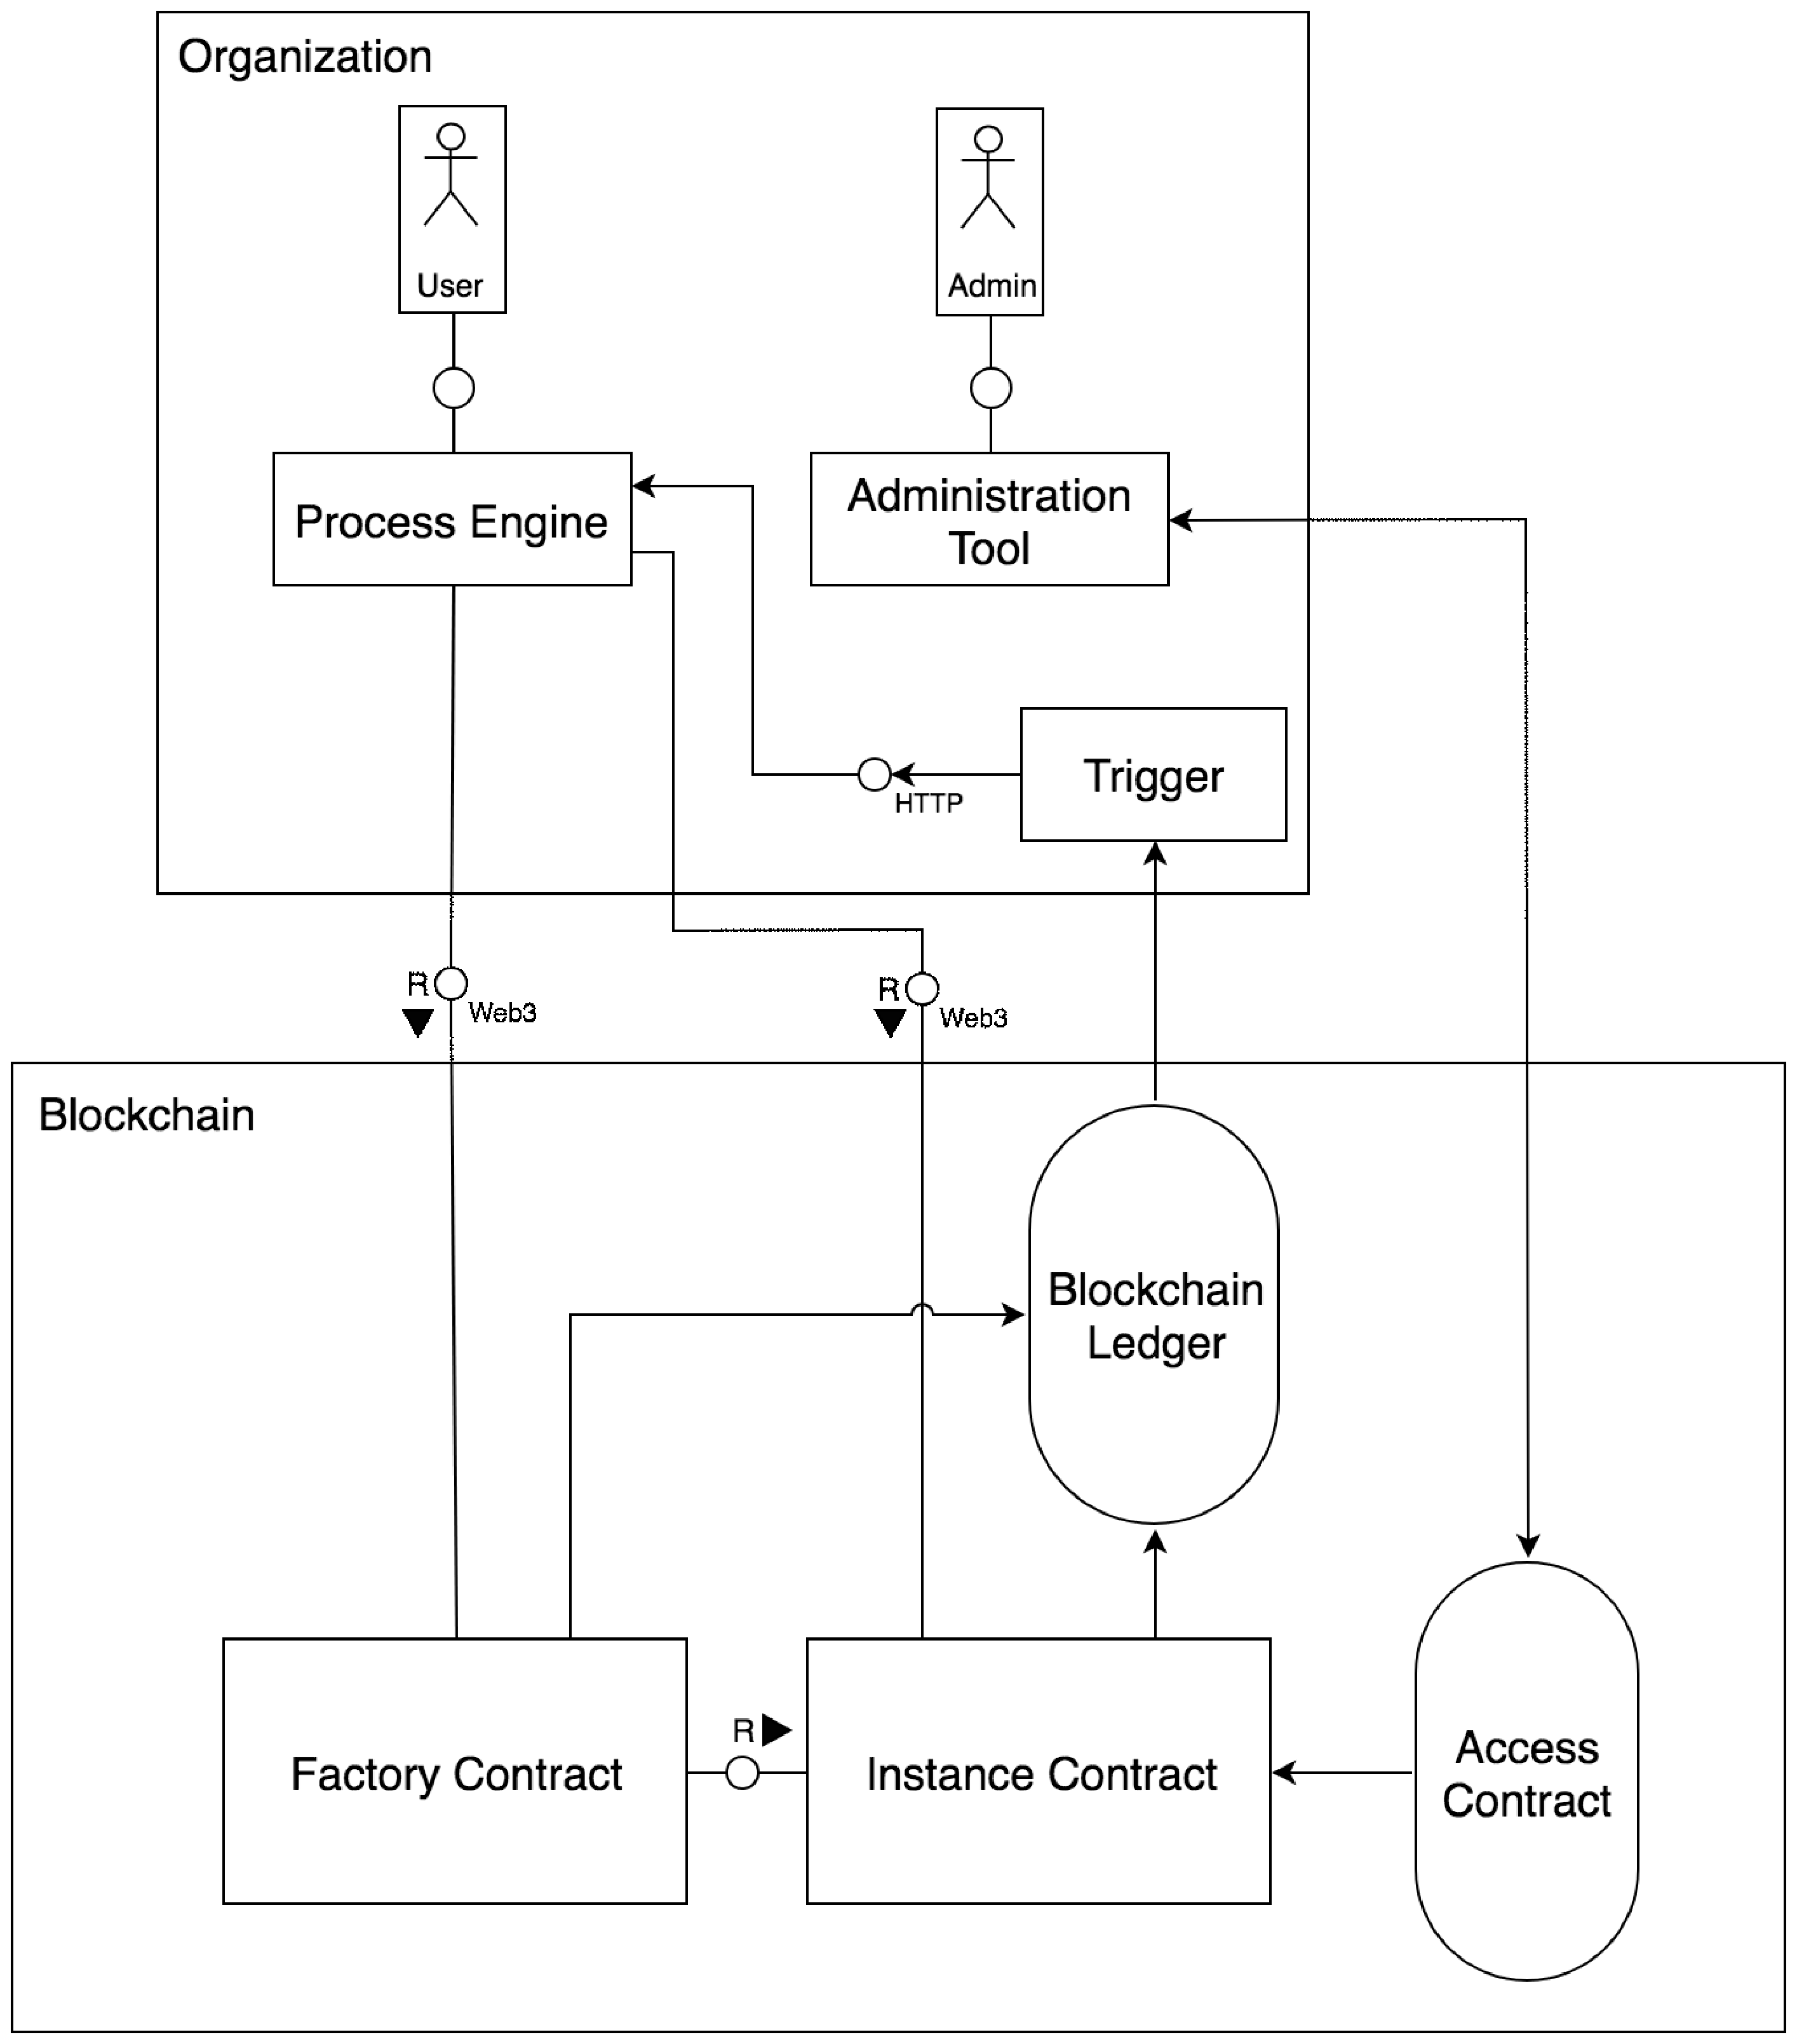
\includegraphics[width=\textwidth]{fig/system_diagram.eps}
\caption{The architecture of our design.} \label{fig1}
\end{figure}

\begin{figure}
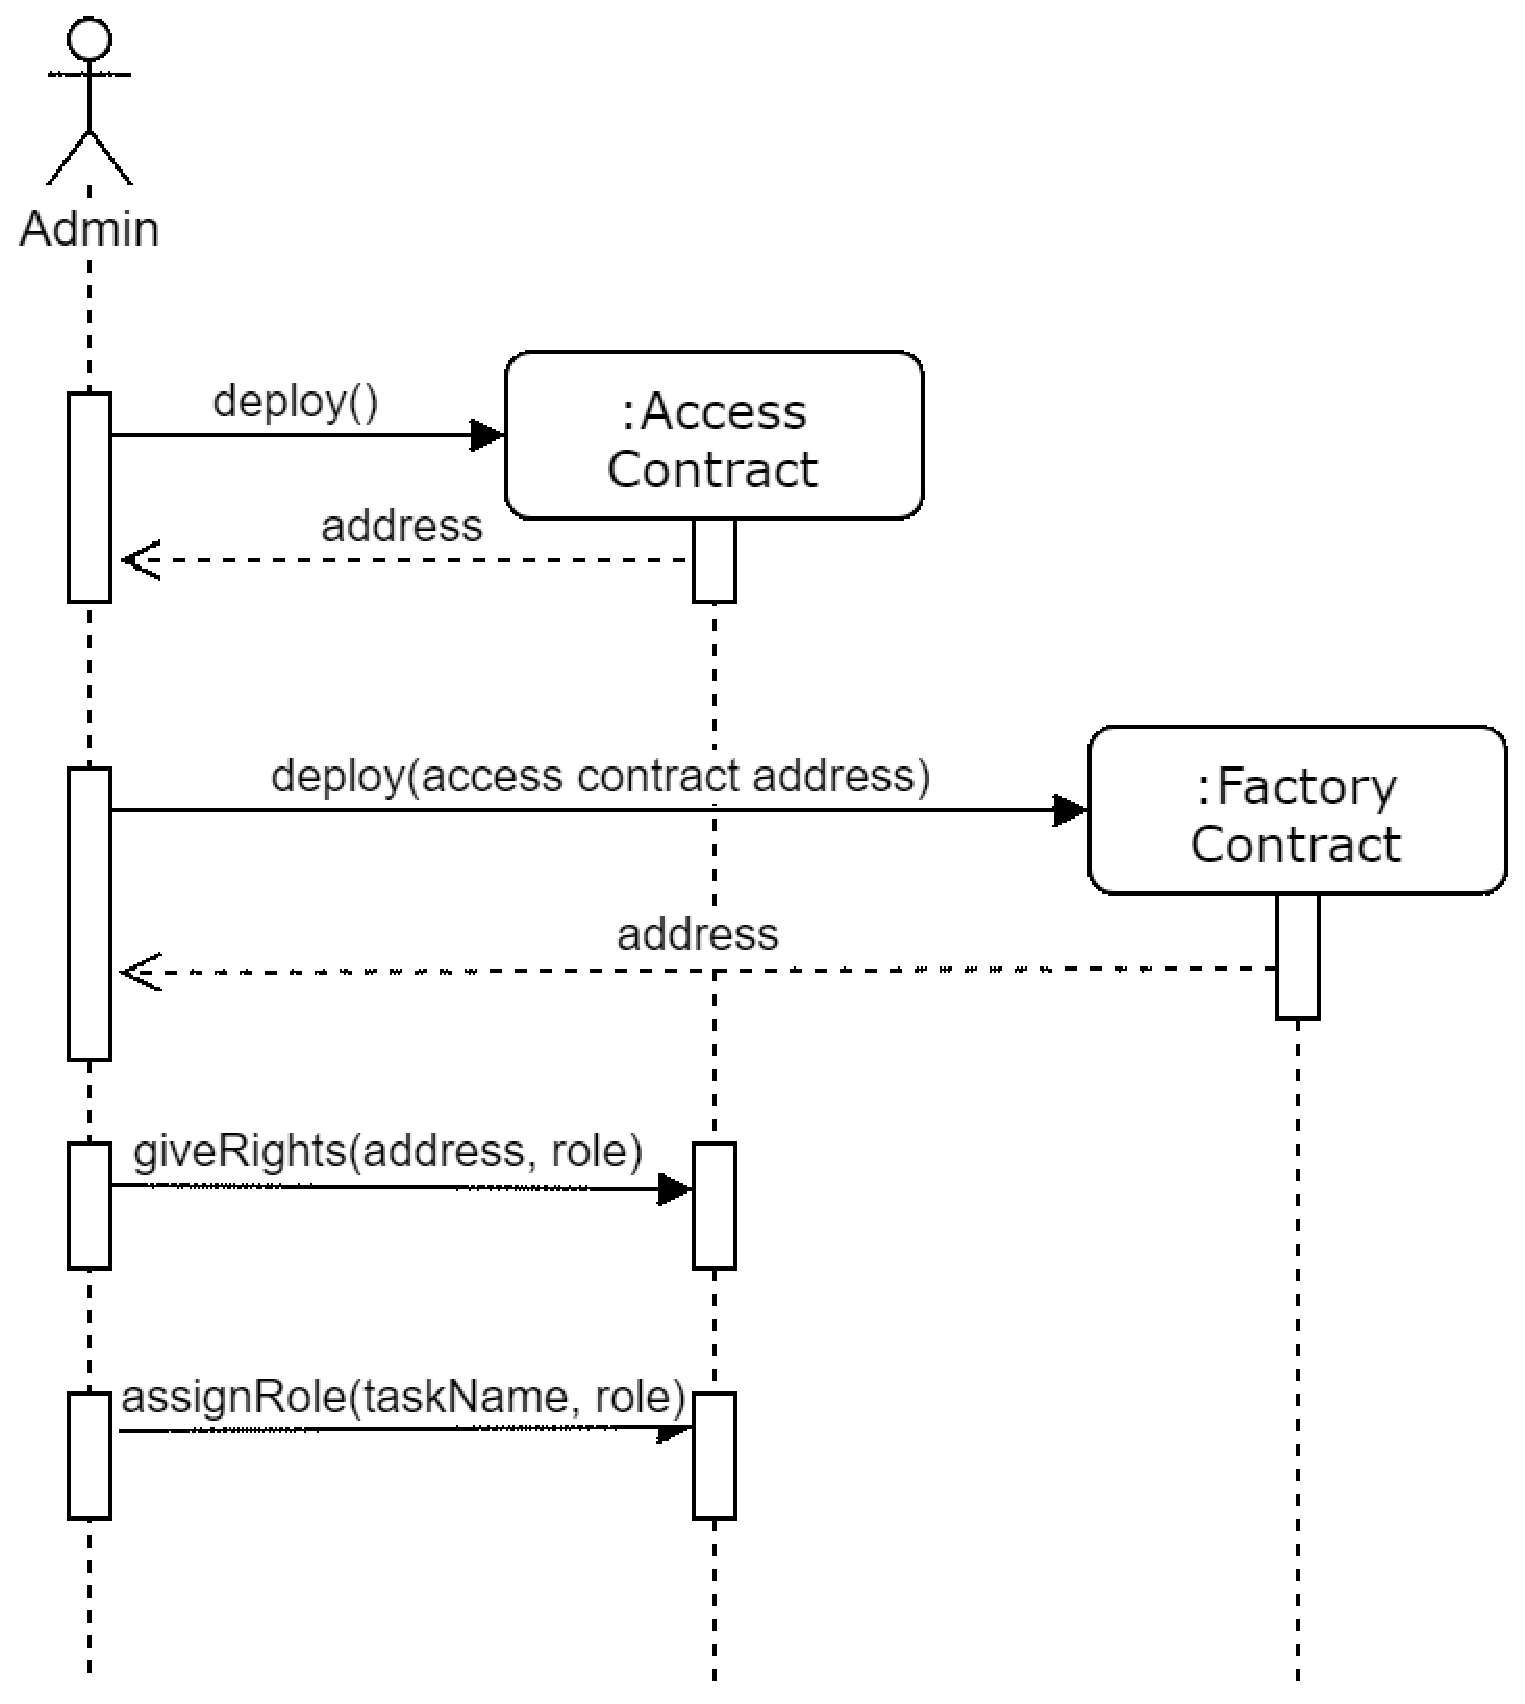
\includegraphics[width=\textwidth]{fig/initialization.eps}
\caption{An initialization process.} \label{fig2}
\end{figure}

\section{Implementation}

\subsection{Contracts}

\subsection{eth\_admin}

\subsection{armadillo}

\section{Evaluation}
%Gas cost
%Time for one instance
%Setup difficulty
%Security

%Mention problem of giving and removing right to change access rights
%But in the end one instance has to a be superadmin in the contract, if it is leaked there is a problem

\section{Conclusion}

%
% ---- Bibliography ----
%
% BibTeX users should specify bibliography style 'splncs04'.
% References will then be sorted and formatted in the correct style.
%
\bibliographystyle{splncs04}
\bibliography{references}

\end{document}
